\chapter{QD Solar Cells}

This chapter gives a brief overview over the fundamental principles of photovoltaic cells and QD solar cells in particular, then focuses on the example of PbS cells to give some specific information.

\section{Solar Cell Principles}

% FIGURE
\begin{figure}
	\centering
	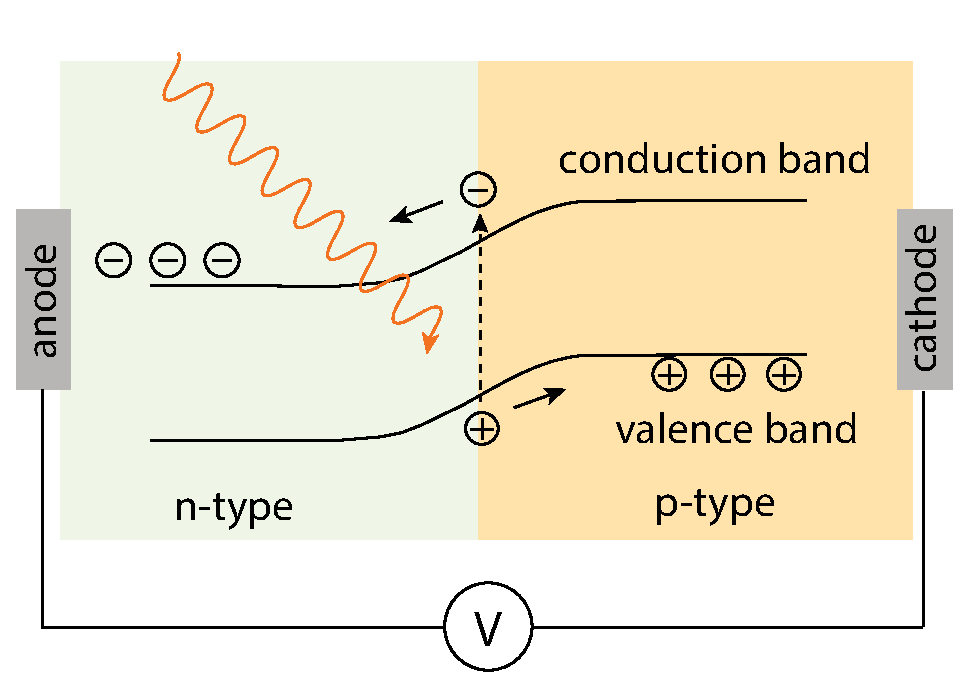
\includegraphics[width=200px]{Fig/SolarCell/pnSolarCell}
	\caption{Principle of a solar cell using a p-n semiconductor junction.}
	\label{fig:pnSolarCell}
\end{figure}

\begin{figure}
	\centering
	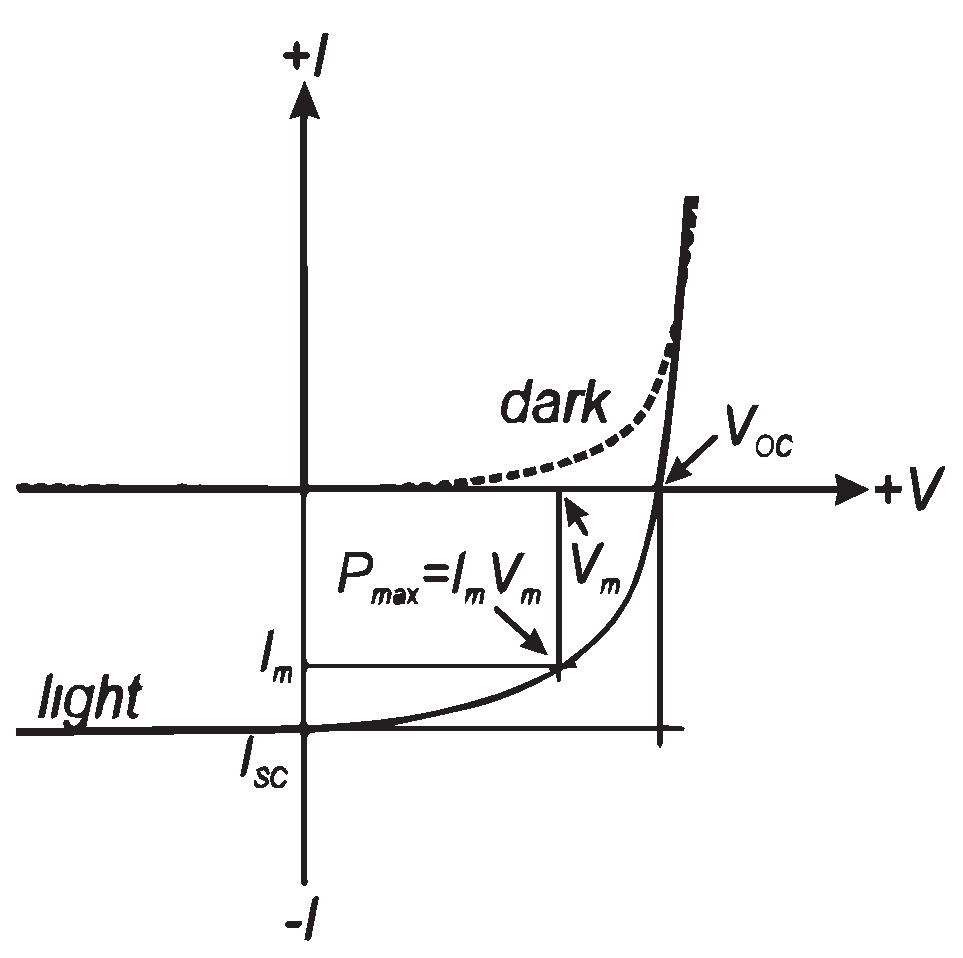
\includegraphics[width=200px]{Fig/SolarCell/IVsolarCell}
	\caption{Typical I-V characteristics of a solar cell. \scshape{Source:} \cite[p.427]{ChemRev}}
	\label{fig:IVsolarCell}
\end{figure}

% TEXT
The basic idea of a solar cell is to convert light into electrical power. Light is absorbed in a material, thus generating an electron-hole pair. The generated electrons and holes must then be separted and conducted to electrodes attached to the material. The accumulation of carriers at the electrodes generates a potential difference, and a current will flow between the electrodes, if a load is connected.

The carrier separation can be achieved by an electric field inside the material. Different types of solar cells exist, based on different approaches. The typical silicon solar cell uses a semiconductor p-n junction: When a photon (with energy greater than the band gap) is absorbed in the semiconductor, an electron is promoted from the valence to the conduction band. Near the junction, these photogenerated electrons and holes are swept away to different sides, due to the built-in electric field of the p-n junction (fig.~\ref{fig:pnSolarCell}). 

Other approaches are also widely used, for example Schottky contacts (metal-semiconductor interface) or semiconductor-liquid interfaces.\\

The electrical behaviour of a photovoltaic cell can be well described by its I-V characteristics (fig.~\ref{fig:IVsolarCell}). In the dark, the cell behaves like a diode (in the case of a p-n junction solar cell this seems fairly obvious). Under illumination, the curve is shifted vertically downwards. It crosses now the fourth quadrant, where the electrical power $P=IV$ is negative, which indicates that power is delivered to the load.\\

To characterise the solar cell, there are some common parameters, which are mentioned in the following paragraph. The open-circuit voltage $V_{OC}$ is the maximum voltage provided by the cell. It is directly related to the energy band structure and thus to the built-in potential. The short-circuit current $I_{SC}$ gives the maximum current, which flows if the electrodes are connected. $I_{SC}$ is proportional to the carrier density under illumination and to the carrier mobility, which are therefore important parameters to maximize.

An often used quantity is the \textit{fill factor (FF)}, which is the ratio between the maximum power $P_M=I_M V_M$ and the product $I_{SC} V_{OC}$. It describes how well behaved the I-V characteristics are (the more the curve approaches a rectangular shape, the better).

Of practical importance for comparing solar cells is the power conversion efficiency $\eta$, giving the ratio of optical power which is converted into electrical power. 
\[\eta = \frac{P_{max}}{P_{in}} = FF\frac{I_{SC}V_{OC}}{P_{in}}\]
Usually an optical source called AM1.5 is used, whose spectral intensity distribution matches that of sunlight reaching the earth's surface at an angle of $48.2^{\circ}$. \cite[pp.426-433]{ChemRev}

\section{Solar Cells using QDs}

Semiconductor nanocrystal solids can be used for solar cells. Thus nanocrystals (NC) made of CdSe, CdTe, PbSe, PbS and many more can be used for this purpose. Like with bulk semiconductors, heterojunction solar cells are possible (using materials with different band gaps), such as CdSe-CdTe cells \cite[p.430]{ChemRev}. Similarly, using Schottky-contacs is also an option.\\

Using NC solids made of QDs offers several advantages. One big advantage is the possibilty of choosing the size of the band gap by controlling the size of the QDs, which can be done easily during the synthesis of CQDs. Controlling the band gap means essentially choosing the spectrum which can be absorbed, and consequently cells, which can make use of a broad spectrum, can be engineered.

Furthermore QD solar cells are easy to fabricate and that at low costs. Large-scale production would also be possible \cite[p.447]{ChemRev}.

Using NC solids, there are promising perspectives for more advanced techniques, in order to increase efficiency. These invlove e.g.~carrier multiplication (the absorption of one highly energetic photon causes the creation of multiple electron-hole pairs) or hot carrier solar cells (electrons in higher energy states in the conduction band are extracted before they relax to the band edge and lose some energy).\\

However, there are some problems which have to be overcome. One is the (air-) stability and lifespan of QD based photovoltaic cells. In many cases, the devices lose dramatically in efficiency after some time, which can be as short as hours or even minutes \cite[p.26]{Tang2011}. Another problem is the currently rather low efficiency of the cells (maxium achieved efficiency of around 7\% for a PbS cell \cite[p.1]{Ip2012}). One issue leading to reduced efficiency is the presence of undesired states in the band gap (mid-gap or trap states). These arise due to `dangling' (unbound) bonds of surface atoms and are significant in a QD, since its surface to volume ratio is high. So-called \textit{passivation} of the surface is thus very important. 

Furthermore, for furture large-scale production, the materials used in the production process should be cheap,  available in large quantities and preferably non-toxic, which contrasts with some NC materials that contain toxic elements like Cd or Pb.

\subsection{Example of a PbS QD Solar Cell}

% FIGURES

\begin{figure}
	\centering
	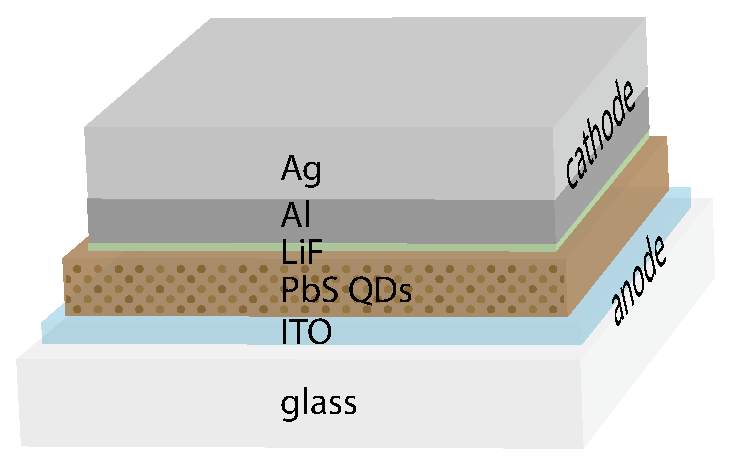
\includegraphics[width=200px]{Fig/SolarCell/PbSsolarCellStructure}
	\caption{Structure of a PbS solar cell.}
	\label{fig:PbSsolarCellStructure}
\end{figure}

% TEXT

Since the structure and fabrication methods of QD solar cell are quite diverse, we will focus here on a PbS QD solar cell, as they were produced at ETH at the Laboratory for Nanoelectronics \cite{MS_Michael}. Due to the small band gap of PbS (0.37eV for bulk PbS), the solar cell is able to convert power from the near infrared spectrum. This is of interest, since roughly 50\% of the solar energy that reaches the earth is in the infrared spectrum.

\subsubsection{Structure}

The principle part of the cell is a Schottky junction of PbS and Al, with a thin protection layer (1 nm) of LiF in between. The Schottky barrier is responsible for the electric field which separates the photogenerated carriers. The Al Cathode is covered by a layer of silver, for better air stability. The transparent anode is formed of a layer of indium tin oxide (ITO), on top of the PbS (fig.~\ref{fig:PbSsolarCellStructure}).

\subsubsection{Fabrication Process}

The main steps involved in the fabrication are described below, as they were carried out in reference \cite[pp. 13-19]{MS_Michael}.

We start with a glass substrate, which is coated with ITO using lithography. The sample has then to be cleaned (using solvents, and afterwards by $O_2$ plasma treatment to remove organic residuals). 

In the next step, the active layer, i.e.~the PbS QDs, is deposited. This can be done by dip coating, where the substrate is immersed in a PbS-hexane solution, and taken out after a few seconds, leaving a thin film of the solution on the sample. Alternatively, spin coating can be used, where several drops of the PbS-Hexane solution are dropped on the substrate, which is then rotated to spread the drops, leading to a film of homogeneous thickness. 

Now the long ligands surrounding the QDs have to be exchanged for short ligands, in order to improve inter-particle coupling (and thus e.g.~carrier mobility). For this purpose, the substrate is immersed into a suitable compound: Ethandithiol, benzenedithiol (both organic), and ammonium thiocyanate ($NH_4SCN$, inorganic) can be used.

The sample is then rinsed in acetonitrile and or hexane. In order to obtain a PbS film of desired thickness, the steps of spin (respectively dip) coating, ligand exchange and rinsing have to be repeated several times.

In a last step, the cathode, i.e.~the three layers of LiF, Al and Ag are evaporated on the substrate.
	